\documentclass[10pt]{standalone}
\usepackage{amsmath,amsfonts,amssymb} % For math equations, theorems, symbols, etc

\usepackage{makecell} % allows line breaking in table cells
\usepackage{pifont}
\usepackage{float}
\usepackage{nameref}
\usepackage[nice]{nicefrac}
\usepackage{marginnote}
\usepackage{stackengine} % needed for \belowbaseline, which is used when aligning matrices by their top row
\usepackage[breakwords]{truncate}
\usepackage{etoolbox} % Needed to make marginnotes always appear in left margin
\newcommand*{\diff}{\mathop{}\:\!d}

\usepackage{graphicx} % Required for including pictures
\usepackage{colortbl}
\arrayrulecolor{gray} % Make block matrices have gray rules

\graphicspath{{images/}} % Specifies the directory where pictures are stored

\usepackage{tikz} % Required for drawing custom shapes
\usepackage{tikz-3dplot} %requires 3dplot.sty to be in same directory, or in your LaTeX installation
\usetikzlibrary{arrows.meta}
\usetikzlibrary{shapes}
\usetikzlibrary{calc,fadings,decorations.pathreplacing,angles,positioning,fit,backgrounds,fpu}
\usepackage{pgfplots}
\pgfplotsset{compat=1.12}
\usepgfplotslibrary{fillbetween}

\newcommand{\RightAngle}[5][3pt]{%
	\draw[#5] ($#3!#1!#2$)
	--($ #3!2!($($#3!#1!#2$)!.5!($#3!#1!#4$)$) $)
	--($#3!#1!#4$) ;
}

\newcommand{\transformarrow}[1]{$\xrightarrow{\ \ \text{#1} \ }$}

% Polynomial long division
\newcommand\Mydiv[2]{%
	\strut#1\kern.25em\smash{\raise.3ex\hbox{\big)}}\mkern-8mu
	\overline{\enspace\strut#2}}

% For drawing graphs in tikz
\tikzstyle{ocrenode}=[draw=ocre,circle,fill=locre,path fading=fade right,text=black,minimum width=10pt]
\tikzstyle{grennode}=[draw=gren,circle,fill=lgren,path fading=fade right,text=black,minimum width=10pt]
\tikzstyle{purpnode}=[draw=purp,circle,fill=lpurp,path fading=fade right,text=black,minimum width=10pt]
\tikzstyle{ocrenoderect}=[draw=ocre,rectangle,rounded corners=5pt,inner sep=6pt,fill=locre,path fading=fade right,text=black,minimum width=10pt]
\tikzstyle{grennoderect}=[draw=gren,rectangle,rounded corners=5pt,inner sep=6pt,fill=lgren,path fading=fade right,text=black,minimum width=10pt]
\tikzstyle{purpnoderect}=[draw=purp,rectangle,rounded corners=5pt,inner sep=6pt,fill=lpurp,path fading=fade right,text=black,minimum width=10pt]
\definecolor{darkorangeback}{RGB}{128,54,0}

\usepackage[english]{babel} % English language/hyphenation
\usepackage{gensymb} % gives the degree symbol

\usepackage{enumitem} % Customize lists
\setlist{nolistsep} % Reduce spacing between bullet points and numbered lists
\usepackage[outline]{contour}

\usepackage{booktabs} % Required for nicer horizontal rules in tables

%% The next command allows for vertical centering of images next to each other in figures.
\newcommand*{\vcenteredhbox}[1]{\begingroup
	\setbox0=\hbox{#1}\parbox{\wd0}{\box0}\endgroup}

\usepackage{multirow} % Used for some subfigure environments when one image is huge
\usepackage{multicol} % Used for enumerate in exercises with multiple images to put them side by side
\usepackage{systeme}\sysdelim.. % Used for typesetting systems of linear equations

\usepackage{xcolor} % Required for specifying colors by name
\usepackage{colortbl}
\definecolor{ocre}{RGB}{0,96,128} % Define the blue color used for highlighting throughout the book
\colorlet{chapcolor}{ocre}
\definecolor{orng}{RGB}{224,112,0} % Define the orange color used for highlighting throughout the book
\definecolor{gren}{RGB}{0,128,0} % Define the green color used for highlighting throughout the book
\definecolor{purp}{RGB}{112,0,112} % Define the purple color used for highlighting throughout the book
\definecolor{dred}{RGB}{164,28,0} % Define the red color used for highlighting throughout the book
\definecolor{locre}{RGB}{128,176,192} % Light blue
\definecolor{lorng}{RGB}{236,184,128} % Light orange
\definecolor{lgren}{RGB}{128,192,128} % Light green
\definecolor{lpurp}{RGB}{184,128,184} % Light purple
\definecolor{lgray}{RGB}{192,192,192} % Light gray
\definecolor{llgray}{RGB}{242,242,242} % Really light (background) gray
\interfootnotelinepenalty=10000 % prevent long footnotes from being split across two pages


% Commands for making letter grids in proofs
\newcommand{\letternode}[3]{\node[anchor=center] at (#1,#2){\fontsize{18}{18}\sffamily\bfseries\contour{black}{\textcolor{ocre!40}{#3}}};}
\newcommand{\colorletternode}[4]{\node[anchor=center] at (#2,#3){\fontsize{18}{18}\sffamily\bfseries\contour{black}{\textcolor{#1!40}{#4}}};}
\newcommand{\sizecolorletternode}[5]{\node[anchor=center] at (#2,#3){\fontsize{#5}{#5}\sffamily\bfseries\contour{black}{\textcolor{#1!40}{#4}}};} 
\newcommand{\gridbox}[2]{\setlength{\fboxsep}{0mm}
	\setlength{\fboxrule}{#1}\fcolorbox{gridgray}{gridgray}{#2}}



% Lets you draw an arc of an ellipse
% From https://tex.stackexchange.com/questions/123158/tikz-using-the-ellipse-command-with-a-start-and-end-angle-instead-of-an-arc
\tikzset{
	partial ellipse/.style args={#1:#2:#3}{
		insert path={+ (#1:#3) arc (#1:#2:#3)}
	}
}


\newcommand{\gliderarrow}[1]{\color{black}{$\xrightarrow{\text{
\includegraphics[width=0.25cm]{../glider.png} #1}}$}}



% DEFINES A GLIDER SHAPE FOR USE IN TIKZ
\def\glider#1#2#3{
	\begin{scope}[shift={#1}, rotate=#2, scale=#3]
		\fill[black](0,0) -- (1,0) -- (1,1) -- (0,1) -- cycle;
		\fill[black](8/7+0,0) -- (8/7+1,0) -- (8/7+1,1) -- (8/7+0,1) -- cycle;
		\fill[black](16/7+0,0) -- (16/7+1,0) -- (16/7+1,1) -- (16/7+0,1) -- cycle;
		\fill[black](16/7+0,8/7+0) -- (16/7+1,8/7+0) -- (16/7+1,8/7+1) -- (16/7+0,8/7+1) -- cycle;
		\fill[black](8/7+0,16/7+0) -- (8/7+1,16/7+0) -- (8/7+1,16/7+1) -- (8/7+0,16/7+1) -- cycle;
\end{scope}}
\def\lwss#1#2#3{
	\begin{scope}[shift={#1}, rotate=#2, scale=#3]
		\fill[black](0,0) -- (1,0) -- (1,1) -- (0,1) -- cycle;
		\fill[black](8/7+0,0) -- (8/7+1,0) -- (8/7+1,1) -- (8/7+0,1) -- cycle;
		\fill[black](16/7+0,0) -- (16/7+1,0) -- (16/7+1,1) -- (16/7+0,1) -- cycle;
		\fill[black](24/7+0,0) -- (24/7+1,0) -- (24/7+1,1) -- (24/7+0,1) -- cycle;
		\fill[black](32/7+0,8/7+0) -- (32/7+1,8/7+0) -- (32/7+1,8/7+1) -- (32/7+0,8/7+1) -- cycle;
		\fill[black](0,8/7+0) -- (1,8/7+0) -- (1,8/7+1) -- (0,8/7+1) -- cycle;
		\fill[black](0,16/7+0) -- (1,16/7+0) -- (1,16/7+1) -- (0,16/7+1) -- cycle;
		\fill[black](8/7+0,24/7+0) -- (8/7+1,24/7+0) -- (8/7+1,24/7+1) -- (8/7+0,24/7+1) -- cycle;
		\fill[black](32/7+0,24/7+0) -- (32/7+1,24/7+0) -- (32/7+1,24/7+1) -- (32/7+0,24/7+1) -- cycle;
\end{scope}}
\def\mwss#1#2#3{
	\begin{scope}[shift={#1}, rotate=#2, scale=#3]
		\fill[black](0,0) -- (1,0) -- (1,1) -- (0,1) -- cycle;
		\fill[black](8/7+0,0) -- (8/7+1,0) -- (8/7+1,1) -- (8/7+0,1) -- cycle;
		\fill[black](16/7+0,0) -- (16/7+1,0) -- (16/7+1,1) -- (16/7+0,1) -- cycle;
		\fill[black](24/7+0,0) -- (24/7+1,0) -- (24/7+1,1) -- (24/7+0,1) -- cycle;
		\fill[black](32/7+0,0) -- (32/7+1,0) -- (32/7+1,1) -- (32/7+0,1) -- cycle;
		\fill[black](40/7+0,8/7+0) -- (40/7+1,8/7+0) -- (40/7+1,8/7+1) -- (40/7+0,8/7+1) -- cycle;
		\fill[black](0,8/7+0) -- (1,8/7+0) -- (1,8/7+1) -- (0,8/7+1) -- cycle;
		\fill[black](0,16/7+0) -- (1,16/7+0) -- (1,16/7+1) -- (0,16/7+1) -- cycle;
		\fill[black](8/7+0,24/7+0) -- (8/7+1,24/7+0) -- (8/7+1,24/7+1) -- (8/7+0,24/7+1) -- cycle;
		\fill[black](24/7+0,32/7+0) -- (24/7+1,32/7+0) -- (24/7+1,32/7+1) -- (24/7+0,32/7+1) -- cycle;
		\fill[black](40/7+0,24/7+0) -- (40/7+1,24/7+0) -- (40/7+1,24/7+1) -- (40/7+0,24/7+1) -- cycle;
\end{scope}}
% DEFINES A BLOCK SHAPE FOR USE IN TIKZ
\def\golblock#1#2#3{
\begin{scope}[shift={#1}, scale=#3]
\fill[#2](0,0) -- (1,0) -- (1,1) -- (0,1) -- cycle;
\fill[#2](8/7+0,0) -- (8/7+1,0) -- (8/7+1,1) -- (8/7+0,1) -- cycle;
\fill[#2](0,8/7+0) -- (1,8/7+0) -- (1,8/7+1) -- (0,8/7+1) -- cycle;
\fill[#2](8/7+0,8/7+0) -- (8/7+1,8/7+0) -- (8/7+1,8/7+1) -- (8/7+0,8/7+1) -- cycle;
\end{scope}}


%----------------------------------------------------------------------------------------
%	FONTS
%----------------------------------------------------------------------------------------

\newcommand{\phantomsectiontotoc}[1]{%
	\addcontentsline{toc}{section}{\protect\numberline{\thesection}{#1}}%
}

% Three colors used in tables
\definecolor{gridgray}{RGB}{192,192,192}
\definecolor{medgray}{RGB}{128,128,128}
\definecolor{redback}{RGB}{255,168,168}
\definecolor{redback2}{RGB}{128,0,0}
\definecolor{greenback}{RGB}{168,255,168}
\definecolor{greenpastel}{RGB}{210,255,210}
\definecolor{greenback2}{RGB}{0,192,0}
\definecolor{darkgreenback}{RGB}{0,96,0}
\definecolor{yellowback}{RGB}{255,255,168}
\definecolor{darkyellowback}{RGB}{96,96,0}
\definecolor{orangeback}{RGB}{255,192,128}
\definecolor{orangeback2}{RGB}{255,220,192}
\definecolor{yellowback2}{RGB}{255,255,192}
\definecolor{aquaback}{RGB}{192,255,255}
\definecolor{darkaquaback}{RGB}{0,96,96}
\definecolor{blueback}{RGB}{168,168,255}
\definecolor{magentaback}{RGB}{255,210,255}
\definecolor{darkmagentaback}{RGB}{96,0,96}
\newcommand{\cmark}{\checkmark} % checkmark
\newcommand{\xmark}{\ding{55}} % matching X

\usepackage{avant} % Use the Avantgarde font for headings
%\usepackage{times} % Use the Times font for headings
\usepackage{mathptmx} % Use the Adobe Times Roman as the default text font together with math symbols from the Sym­bol, Chancery and Com­puter Modern fonts

\usepackage{microtype} % Slightly tweak font spacing for aesthetics
\usepackage[utf8]{inputenc} % Required for including letters with accents
\usepackage[T1]{fontenc} % Use 8-bit encoding that has 256 glyphs

\usepackage{calc} % For simpler calculation - used for spacing the index letter headings correctly


\DeclareMathAlphabet{\mathcal}{OMS}{cmsy}{m}{n} % Resets \mathcal to the usual mathcal font (used for subspaces, for example)
\def\C{\mathbb{C}}
\def\N{\mathbb{N}}
\def\Q{\mathbb{Q}}
\def\R{\mathbb{R}}

\def\B{\mathcal{B}}
\def\S{\mathcal{S}}
\def\U{\mathcal{U}}
\def\V{\mathcal{V}}
\def\W{\mathcal{W}}
\def\X{\mathcal{X}}

\def\a{\mathbf{a}}
\def\b{\mathbf{b}}
\def\c{\mathbf{c}}
\def\d{\mathbf{d}}
\def\e{\mathbf{e}}
\def\p{\mathbf{p}}
\def\r{\mathbf{r}}
\def\u{\mathbf{u}}
\def\v{\mathbf{v}}
\def\w{\mathbf{w}}
\def\x{\mathbf{x}}
\def\y{\mathbf{y}}
\def\z{\mathbf{z}}
\def\0{\mathbf{0}}

\def\range{\operatorname{range}}
\def\rank{\operatorname{rank}}
\def\nullity{\operatorname{nullity}}
\def\mat{\mathrm{mat}}
\newcommand{\tr}{\mathrm{tr}}
\def\vecop{\mathrm{vec}} % do NOT redefine as \vec -- you want that command to put an arrow over a vector

\def\CNOT{\mathrm{CNOT}}
\def\NOT{\mathrm{NOT}}
\def\AND{\mathrm{AND}}
\newcommand{\smallaug}[2]{[ \ #1 \ {\color{gray}|} \ #2 \ ]}

\def\smashddots{\vphantom{\int^0}\smash[t]{\ddots}}
\def\smashvdots{\vphantom{\int^0}\smash[t]{\vdots}}
\def\nullspace{\operatorname{null}}


% COMMAND FOR ROW OPERATIONS
\newcommand\rowop[1]{\raisebox{-0.3\height}{$\xrightarrow{#1}$}}
\newcommand\ip[2]{\ensuremath{\langle#1,#2\rangle}}


\tikzfading[name=fade right,left color=transparent!20, right color=transparent!70,shading angle=140]
\tikzfading[name=fade left,left color=transparent!20, right color=transparent!70,shading angle=220]
\tikzfading[name=fade bottom,left color=transparent!20, right color=transparent!70,shading angle=30]


\begin{document}
	\begin{tikzpicture}%
		\node[inner sep=0pt,anchor=south west] (rp) at (0,0) {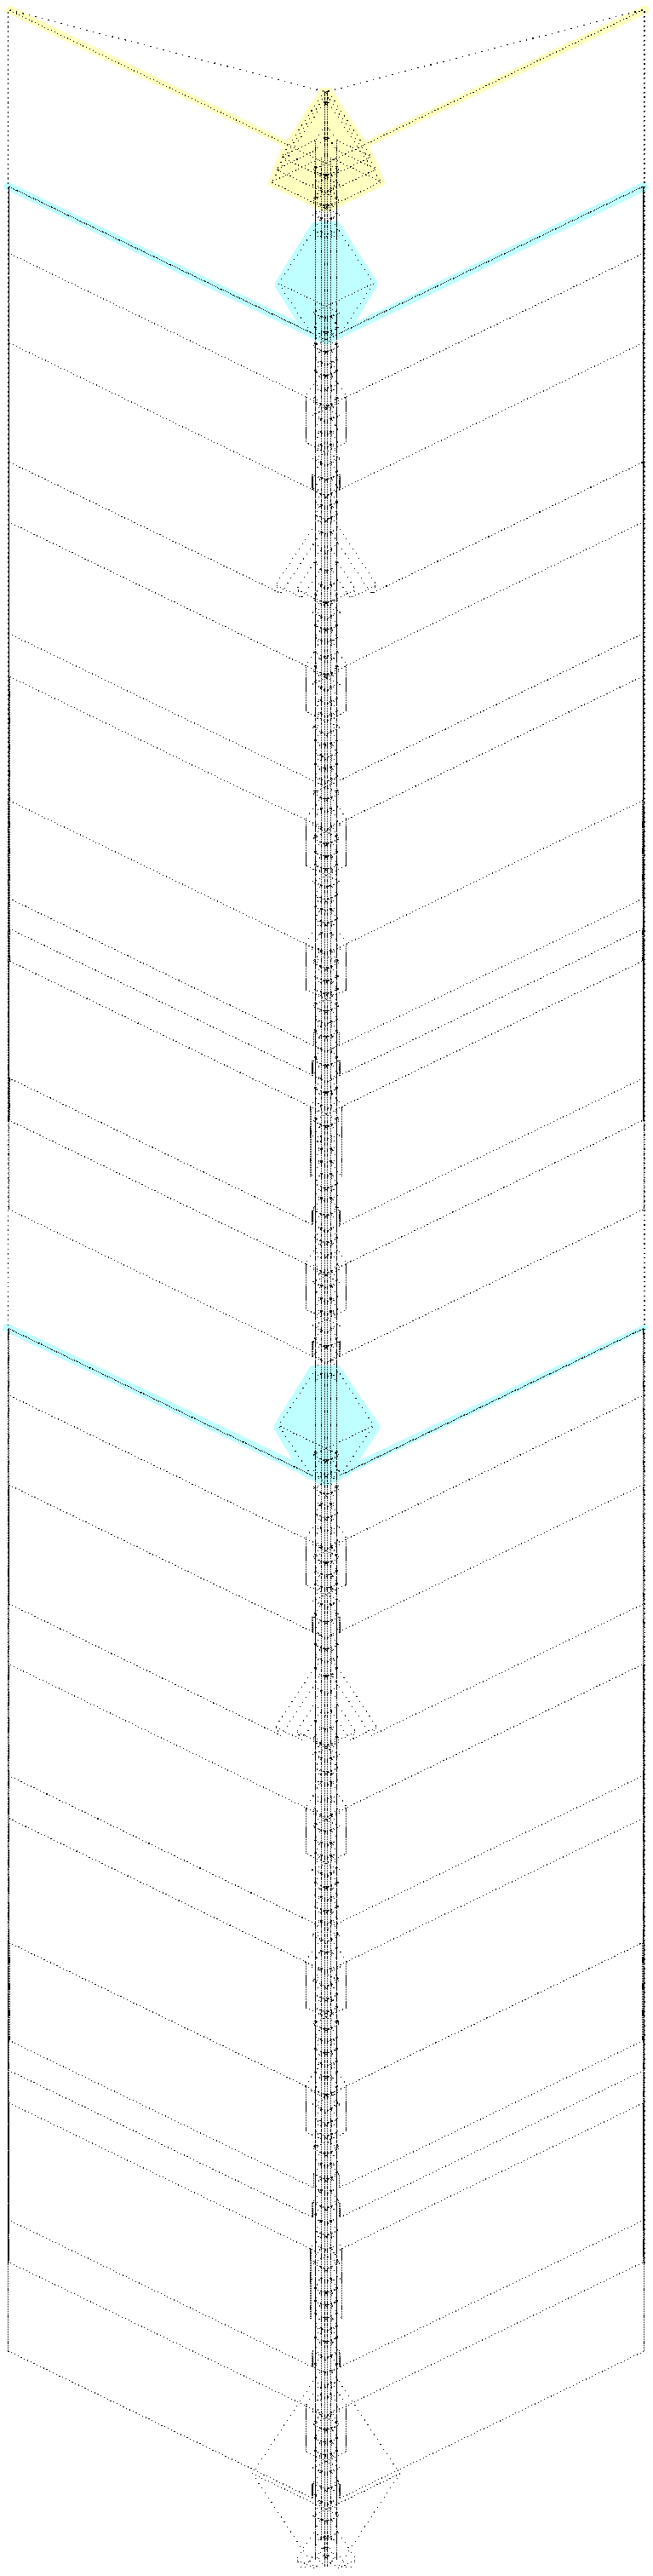
\includegraphics[width=4.5cm]{silverfish.png}};
		
		% FIRST RAKE
		\newcommand\rakeonex{3.2}
		\newcommand\rakeoney{7.64}
		\draw[gray] (\rakeonex,\rakeoney+0.03) node[rotate=24] {\tiny \texttt{R6L6}};
		\draw[color=gray,-stealth] (\rakeonex-0.23,\rakeoney-0.18) -- (\rakeonex+0.38,\rakeoney+0.11);
		
		% 2nd RAKE
		\newcommand\raketwox{3.2}
		\newcommand\raketwoy{7.03}
		\draw[gray] (\raketwox,\raketwoy+0.03) node[rotate=24] {\tiny \texttt{R2L25}};
		\draw[color=gray,-stealth] (\raketwox-0.23,\raketwoy-0.18) -- (\raketwox+0.38,\raketwoy+0.11);
		
		% 3rd RAKE
		\newcommand\rakethreex{3.2}
		\newcommand\rakethreey{6.2}
		\draw[gray] (\rakethreex,\rakethreey+0.03) node[rotate=24] {\tiny \texttt{R6L17}};
		\draw[color=gray,-stealth] (\rakethreex-0.23,\rakethreey-0.18) -- (\rakethreex+0.38,\rakethreey+0.11);
		
		% 4th RAKE
		\newcommand\rakefourx{3.2}
		\newcommand\rakefoury{5.78}
		\draw[gray] (\rakefourx,\rakefoury+0.03) node[rotate=24] {\tiny \texttt{R6L6}};
		\draw[color=gray,-stealth] (\rakefourx-0.23,\rakefoury-0.18) -- (\rakefourx+0.38,\rakefoury+0.11);
		
		% 5th RAKE
		\newcommand\rakefivex{3.2}
		\newcommand\rakefivey{5.02}
		\draw[gray] (\rakefivex,\rakefivey+0.03) node[rotate=24] {\tiny \texttt{R1L0}};
		\draw[color=gray,-stealth] (\rakefivex-0.23,\rakefivey-0.18) -- (\rakefivex+0.38,\rakefivey+0.11);
		
		% 6th RAKE
		\newcommand\rakesixx{3.2}
		\newcommand\rakesixy{4.73}
		\draw[gray] (\rakesixx,\rakesixy+0.03) node[rotate=24] {\tiny \texttt{R6L6}};
		\draw[color=gray,-stealth] (\rakesixx-0.23,\rakesixy-0.18) -- (\rakesixx+0.38,\rakesixy+0.11);
		
		% 7th RAKE
		\newcommand\rakesevenx{3.2}
		\newcommand\rakeseveny{3.87}
		\draw[gray] (\rakesevenx,\rakeseveny+0.03) node[rotate=24] {\tiny \texttt{R6L6}};
		\draw[color=gray,-stealth] (\rakesevenx-0.23,\rakeseveny-0.18) -- (\rakesevenx+0.38,\rakeseveny+0.11);
		
		% 8th RAKE
		\newcommand\rakeeightx{2.9}
		\newcommand\rakeeighty{3.05}
		\draw[gray] (\rakeeightx,\rakeeighty+0.03) node[rotate=24] {\tiny \texttt{R2L23}};
		\draw[color=gray,-stealth] (\rakeeightx-0.23,\rakeeighty-0.18) -- (\rakeeightx+0.38,\rakeeighty+0.11);
		
		% 9th RAKE
		\newcommand\rakeninex{3.7}
		\newcommand\rakeniney{3.15}
		\draw[gray] (\rakeninex+0.09,\rakeniney-0.15) node[rotate=24] {\tiny \texttt{R2L25}};
		\draw[color=gray,-stealth] (\rakeninex-0.23,\rakeniney-0.18) -- (\rakeninex+0.38,\rakeniney+0.11);
		
		% 10th RAKE
		\newcommand\raketenx{3.2}
		\newcommand\raketeny{2.45}
		\draw[gray] (\raketenx,\raketeny+0.03) node[rotate=24] {\tiny \texttt{R2L25}};
		\draw[color=gray,-stealth] (\raketenx-0.23,\raketeny-0.18) -- (\raketenx+0.38,\raketeny+0.11);
		
		% 11th RAKE
		\newcommand\rakeelevenx{3.2}
		\newcommand\rakeeleveny{1.97}
		\draw[gray] (\rakeelevenx,\rakeeleveny+0.03) node[rotate=24] {\tiny \texttt{R2L25}};
		\draw[color=gray,-stealth] (\rakeelevenx-0.23,\rakeeleveny-0.18) -- (\rakeelevenx+0.38,\rakeeleveny+0.11);
		
		% 12th RAKE
		\newcommand\raketwelvex{3.2}
		\newcommand\raketwelvey{1.68}
		\draw[gray] (\raketwelvex,\raketwelvey+0.03) node[rotate=24] {\tiny \texttt{R6L6}};
		\draw[color=gray,-stealth] (\raketwelvex-0.23,\raketwelvey-0.18) -- (\raketwelvex+0.38,\raketwelvey+0.11);
		
		% 13th RAKE
		\newcommand\rakethirteenx{3.2}
		\newcommand\rakethirteeny{1.07}
		\draw[gray] (\rakethirteenx,\rakethirteeny+0.03) node[rotate=24] {\tiny \texttt{R2L25}};
		\draw[color=gray,-stealth] (\rakethirteenx-0.23,\rakethirteeny-0.18) -- (\rakethirteenx+0.38,\rakethirteeny+0.11);
		
%		% BORDER
%		\draw[gridgray] (0,0) rectangle (12,17.78);
%		\clip (0,0) rectangle (12,17.78);
%		
		% ZOOM BOX 1
			\newcommand\smlx{4.36}
			\newcommand\smrx{\smlx+0.2}
			\newcommand\smby{17.57}
			\newcommand\smty{\smby+0.2}
			
			\newcommand\bglx{9}
			\newcommand\bgrx{\bglx+3}
			\newcommand\bgty{17.5}
			\newcommand\bgby{\bgty-3}
			
			\path[draw,gridgray,line width=0.45pt] (\smrx,\smty) -- (\bgrx,\bgty);
			\path[draw,gridgray,line width=0.45pt] (\smrx,\smby) -- (\bgrx,\bgby);
			
			\node[inner sep=0pt,anchor=north west] (zoom1) at (\bglx,\bgty) {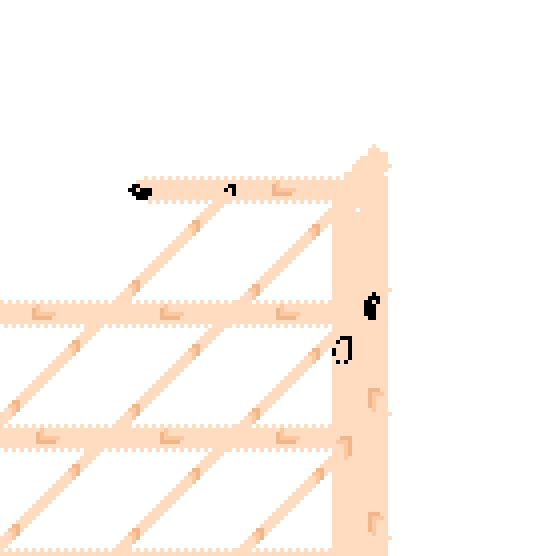
\includegraphics[width=3cm]{silverfish_top_right.png}};
			
			\path[fill,white,opacity=0.4,line width=0pt] (\smrx,\smty) -- (\smlx,\smty) -- (\bglx,\bgty) -- (\bglx,\bgby) -- (\smlx,\smby)-- (\smrx,\smby) -- cycle;
			
			%\node[inner sep=0pt] (zoom1_3x) at (3.35,7.95) {
\includegraphics[width=0.21cm]{../mag.png} \footnotesize 8x};
			
			\filldraw[draw=gridgray,fill=white,line width=0.3pt,fill opacity=0.64] (\smlx,\smty) rectangle (\smrx,\smby);
			\draw[gridgray,line width=0.6pt] (\bglx,\bgty) rectangle (\bgrx,\bgby);
			\path[draw,gridgray,line width=0.45pt] (\smlx,\smby) -- (\bglx,\bgby);
			\path[draw,gridgray,line width=0.45pt] (\smlx,\smty) -- (\bglx,\bgty);
		% END ZOOM BOX 1

		% ZOOM BOX 2
			\newcommand\twosmlx{2.165}
			\newcommand\twosmrx{\twosmlx+0.2}
			\newcommand\twosmby{17.03}
			\newcommand\twosmty{\twosmby+0.2}
			
			\newcommand\twobglx{5.25}
			\newcommand\twobgrx{\twobglx+3}
			\newcommand\twobgty{17}
			\newcommand\twobgby{\twobgty-3}
			
			\path[draw,gridgray,line width=0.45pt] (\twosmrx,\twosmby) -- (\twobgrx,\twobgby);
			
			\node[inner sep=0pt,anchor=north west] (zoom2) at (\twobglx,\twobgty) {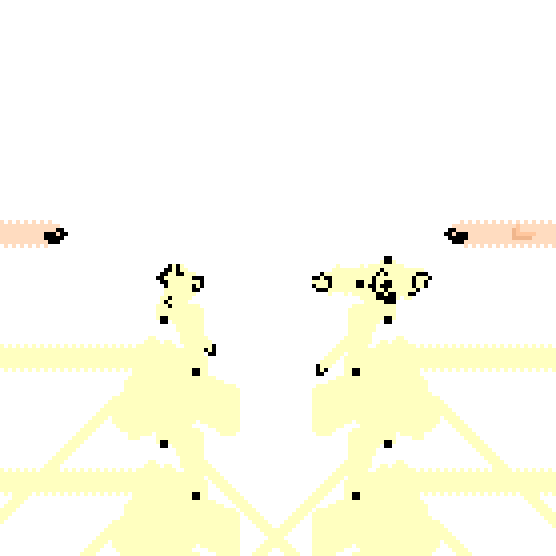
\includegraphics[width=3cm]{silverfish_top_center.png}};
			
			\path[fill,white,opacity=0.4,line width=0pt] (\twosmrx,\twosmty) -- (\twobgrx,\twobgty) -- (\twobglx,\twobgty) -- (\twobglx,\twobgby) -- (\twosmlx,\twosmby)-- (\twosmrx,\twosmby) -- cycle;
			
			%\node[inner sep=0pt] (zoom1_3x) at (3.35,7.95) {
\includegraphics[width=0.21cm]{../mag.png} \footnotesize 8x};
			
			\filldraw[draw=gridgray,fill=white,line width=0.3pt,fill opacity=0.64] (\twosmlx,\twosmty) rectangle (\twosmrx,\twosmby);
			\draw[gridgray,line width=0.6pt] (\twobglx,\twobgty) rectangle (\twobgrx,\twobgby);
			\path[draw,gridgray,line width=0.45pt] (\twosmrx,\twosmty) -- (\twobgrx,\twobgty);
			\path[draw,gridgray,line width=0.45pt] (\twosmlx,\twosmby) -- (\twobglx,\twobgby);
			\path[draw,gridgray,line width=0.45pt] (\twosmlx,\twosmty) -- (\twobglx,\twobgty);
		% END ZOOM BOX 2
		
		% ZOOM BOX SYNTH1
			\newcommand\thrsmlx{4.36}
			\newcommand\thrsmrx{\thrsmlx+0.2}
			\newcommand\thrsmby{8.5}
			\newcommand\thrsmty{\thrsmby+0.2}
			
			\newcommand\thrbglx{5.25}
			\newcommand\thrbgrx{\thrbglx+2}
			\newcommand\thrbgty{12.5}
			\newcommand\thrbgby{\thrbgty-2}
			
			\node[inner sep=0pt,anchor=north west] (zooms1) at (\thrbglx,\thrbgty) {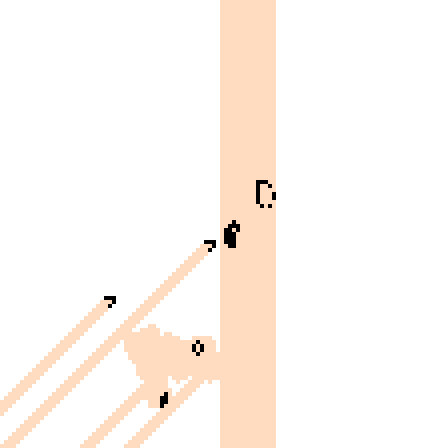
\includegraphics[width=2cm]{silverfish_synth1.png}};
			
			\filldraw[draw=gridgray,fill=white,line width=0.3pt,fill opacity=0.8] (\thrsmlx,\thrsmty) rectangle (\thrsmrx,\thrsmby);
			\draw[gridgray,line width=0.6pt] (\thrbglx,\thrbgty) rectangle (\thrbgrx,\thrbgby);
			
			\draw[gray] (\thrsmlx+0.1,\thrsmty-0.1) node {\tiny \texttt{1}};
			\draw[gray] (\thrbglx,\thrbgty) node[anchor=north west] {\small \texttt{1}};
		% END ZOOM SYNTH1
		
		% ZOOM BOX SYNTH2
			\newcommand\syntwosmlx{4.36}
			\newcommand\syntwosmrx{\syntwosmlx+0.2}
			\newcommand\syntwosmby{8.02}
			\newcommand\syntwosmty{\syntwosmby+0.2}
			
			\newcommand\syntwobglx{7.625}
			\newcommand\syntwobgrx{\syntwobglx+2}
			\newcommand\syntwobgty{12.5}
			\newcommand\syntwobgby{\syntwobgty-2}
			
			\node[inner sep=0pt,anchor=north west] (zooms2) at (\syntwobglx,\syntwobgty) {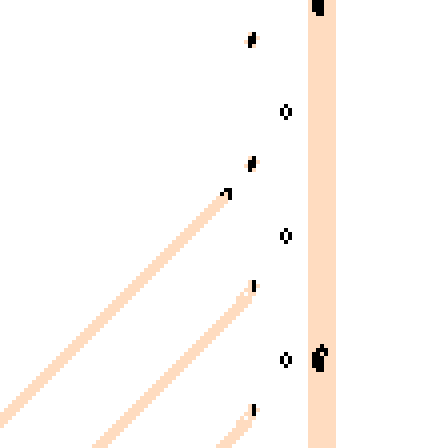
\includegraphics[width=2cm]{silverfish_synth2.png}};
			
			\filldraw[draw=gridgray,fill=white,line width=0.3pt,fill opacity=0.8] (\syntwosmlx,\syntwosmty) rectangle (\syntwosmrx,\syntwosmby);
			\draw[gridgray,line width=0.6pt] (\syntwobglx,\syntwobgty) rectangle (\syntwobgrx,\syntwobgby);
			
			\draw[gray] (\syntwosmlx+0.1,\syntwosmty-0.1) node {\tiny \texttt{2}};
			\draw[gray] (\syntwobglx,\syntwobgty) node[anchor=north west] {\small \texttt{2}};
		% END ZOOM SYNTH2
		
		% ZOOM BOX SYNTH3
			\newcommand\synthreesmlx{4.36}
			\newcommand\synthreesmrx{\synthreesmlx+0.2}
			\newcommand\synthreesmby{7.42}
			\newcommand\synthreesmty{\synthreesmby+0.2}
			
			\newcommand\synthreebglx{10}
			\newcommand\synthreebgrx{\synthreebglx+2}
			\newcommand\synthreebgty{12.5}
			\newcommand\synthreebgby{\synthreebgty-2}
			
			\node[inner sep=0pt,anchor=north west] (zooms3) at (\synthreebglx,\synthreebgty) {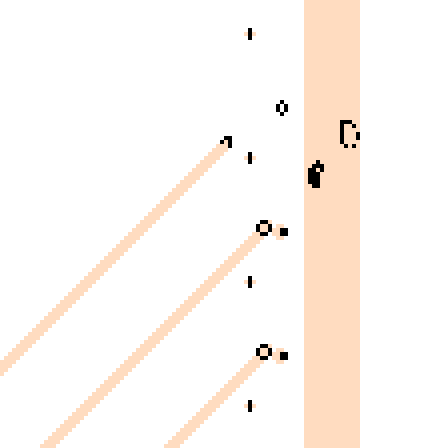
\includegraphics[width=2cm]{silverfish_synth3.png}};
			
			\filldraw[draw=gridgray,fill=white,line width=0.3pt,fill opacity=0.8] (\synthreesmlx,\synthreesmty) rectangle (\synthreesmrx,\synthreesmby);
			\draw[gridgray,line width=0.6pt] (\synthreebglx,\synthreebgty) rectangle (\synthreebgrx,\synthreebgby);
			
			\draw[gray] (\synthreesmlx+0.1,\synthreesmty-0.1) node {\tiny \texttt{3}};
			\draw[gray] (\synthreebglx,\synthreebgty) node[anchor=north west] {\small \texttt{3}};
		% END ZOOM SYNTH3
		
		% ZOOM BOX SYNTH4
			\newcommand\synfoursmlx{4.36}
			\newcommand\synfoursmrx{\synfoursmlx+0.2}
			\newcommand\synfoursmby{6.6}
			\newcommand\synfoursmty{\synfoursmby+0.2}
			
			\newcommand\synfourbglx{5.25}
			\newcommand\synfourbgrx{\synfourbglx+2}
			\newcommand\synfourbgty{10.125}
			\newcommand\synfourbgby{\synfourbgty-2}
			
			\node[inner sep=0pt,anchor=north west] (zooms4) at (\synfourbglx,\synfourbgty) {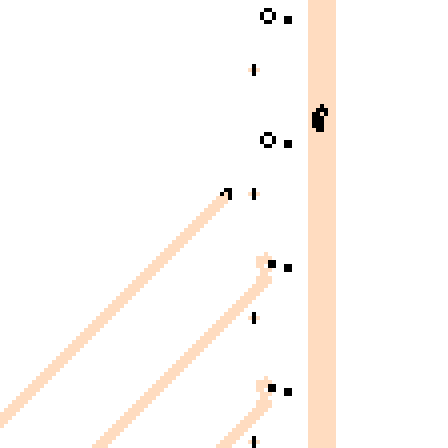
\includegraphics[width=2cm]{silverfish_synth4.png}};
			
			\filldraw[draw=gridgray,fill=white,line width=0.3pt,fill opacity=0.8] (\synfoursmlx,\synfoursmty) rectangle (\synfoursmrx,\synfoursmby);
			\draw[gridgray,line width=0.6pt] (\synfourbglx,\synfourbgty) rectangle (\synfourbgrx,\synfourbgby);
			
			\draw[gray] (\synfoursmlx+0.1,\synfoursmty-0.1) node {\tiny \texttt{4}};
			\draw[gray] (\synfourbglx,\synfourbgty) node[anchor=north west] {\small \texttt{4}};
		% END ZOOM SYNTH4
		
		% ZOOM BOX SYNTH5
			\newcommand\synfivesmlx{4.36}
			\newcommand\synfivesmrx{\synfivesmlx+0.2}
			\newcommand\synfivesmby{6.19}
			\newcommand\synfivesmty{\synfivesmby+0.2}
			
			\newcommand\synfivebglx{7.625}
			\newcommand\synfivebgrx{\synfivebglx+2}
			\newcommand\synfivebgty{10.125}
			\newcommand\synfivebgby{\synfivebgty-2}
			
			\node[inner sep=0pt,anchor=north west] (zooms5) at (\synfivebglx,\synfivebgty) {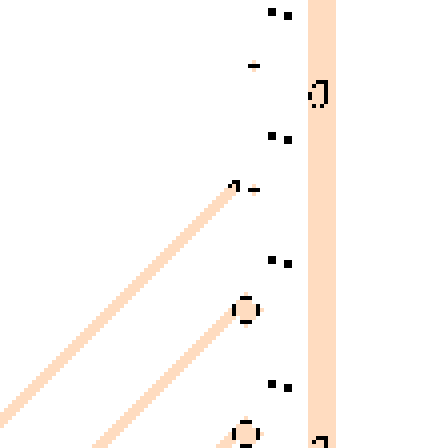
\includegraphics[width=2cm]{silverfish_synth5.png}};
			
			\filldraw[draw=gridgray,fill=white,line width=0.3pt,fill opacity=0.8] (\synfivesmlx,\synfivesmty) rectangle (\synfivesmrx,\synfivesmby);
			\draw[gridgray,line width=0.6pt] (\synfivebglx,\synfivebgty) rectangle (\synfivebgrx,\synfivebgby);
			
			\draw[gray] (\synfivesmlx+0.1,\synfivesmty-0.1) node {\tiny \texttt{5}};
			\draw[gray] (\synfivebglx,\synfivebgty) node[anchor=north west] {\small \texttt{5}};
		% END ZOOM SYNTH5
		
		% ZOOM BOX SYNTH6
			\newcommand\synsixsmlx{4.36}
			\newcommand\synsixsmrx{\synsixsmlx+0.2}
			\newcommand\synsixsmby{5.43}
			\newcommand\synsixsmty{\synsixsmby+0.2}
			
			\newcommand\synsixbglx{10}
			\newcommand\synsixbgrx{\synsixbglx+2}
			\newcommand\synsixbgty{10.125}
			\newcommand\synsixbgby{\synsixbgty-2}
			
			\node[inner sep=0pt,anchor=north west] (zooms6) at (\synsixbglx,\synsixbgty) {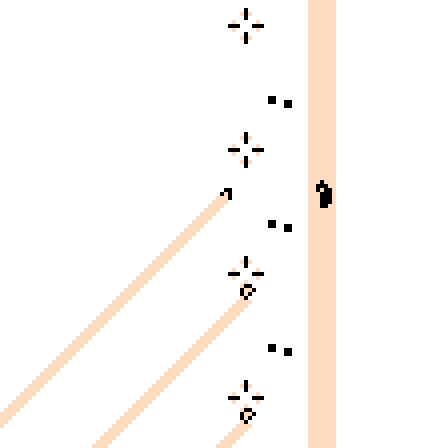
\includegraphics[width=2cm]{silverfish_synth6.png}};
			
			\filldraw[draw=gridgray,fill=white,line width=0.3pt,fill opacity=0.8] (\synsixsmlx,\synsixsmty) rectangle (\synsixsmrx,\synsixsmby);
			\draw[gridgray,line width=0.6pt] (\synsixbglx,\synsixbgty) rectangle (\synsixbgrx,\synsixbgby);
			
			\draw[gray] (\synsixsmlx+0.1,\synsixsmty-0.1) node {\tiny \texttt{6}};
			\draw[gray] (\synsixbglx,\synsixbgty) node[anchor=north west] {\small \texttt{6}};
		% END ZOOM SYNTH6

		% ZOOM BOX SYNTH7
			\newcommand\synsevensmlx{4.36}
			\newcommand\synsevensmrx{\synsevensmlx+0.2}
			\newcommand\synsevensmby{5.12}
			\newcommand\synsevensmty{\synsevensmby+0.2}
			
			\newcommand\synsevenbglx{5.25}
			\newcommand\synsevenbgrx{\synsevenbglx+2}
			\newcommand\synsevenbgty{7.75}
			\newcommand\synsevenbgby{\synsevenbgty-2}
			
			\node[inner sep=0pt,anchor=north west] (zooms7) at (\synsevenbglx,\synsevenbgty) {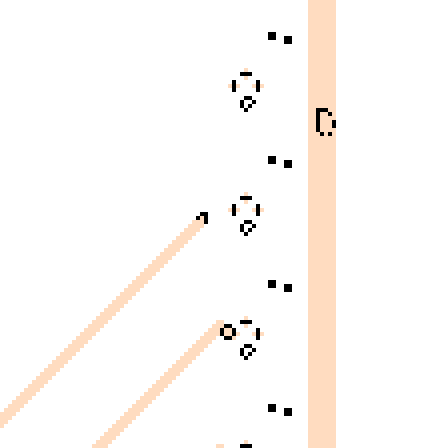
\includegraphics[width=2cm]{silverfish_synth7.png}};
			
			\filldraw[draw=gridgray,fill=white,line width=0.3pt,fill opacity=0.8] (\synsevensmlx,\synsevensmty) rectangle (\synsevensmrx,\synsevensmby);
			\draw[gridgray,line width=0.6pt] (\synsevenbglx,\synsevenbgty) rectangle (\synsevenbgrx,\synsevenbgby);
			
			\draw[gray] (\synsevensmlx+0.1,\synsevensmty-0.1) node {\tiny \texttt{7}};
			\draw[gray] (\synsevenbglx,\synsevenbgty) node[anchor=north west] {\small \texttt{7}};
		% END ZOOM SYNTH7
		
		% ZOOM BOX SYNTH8
			\newcommand\syneightsmlx{4.36}
			\newcommand\syneightsmrx{\syneightsmlx+0.2}
			\newcommand\syneightsmby{4.27}
			\newcommand\syneightsmty{\syneightsmby+0.2}
			
			\newcommand\syneightbglx{7.625}
			\newcommand\syneightbgrx{\syneightbglx+2}
			\newcommand\syneightbgty{7.75}
			\newcommand\syneightbgby{\syneightbgty-2}
			
			\node[inner sep=0pt,anchor=north west] (zooms8) at (\syneightbglx,\syneightbgty) {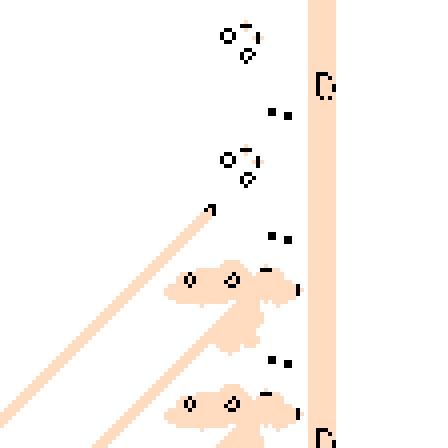
\includegraphics[width=2cm]{silverfish_synth8.png}};
			
			\filldraw[draw=gridgray,fill=white,line width=0.3pt,fill opacity=0.8] (\syneightsmlx,\syneightsmty) rectangle (\syneightsmrx,\syneightsmby);
			\draw[gridgray,line width=0.6pt] (\syneightbglx,\syneightbgty) rectangle (\syneightbgrx,\syneightbgby);
			
			\draw[gray] (\syneightsmlx+0.1,\syneightsmty-0.1) node {\tiny \texttt{8}};
			\draw[gray] (\syneightbglx,\syneightbgty) node[anchor=north west] {\small \texttt{8}};
		% END ZOOM SYNTH8
		
		% ZOOM BOX SYNTH9
			\newcommand\synninesmlx{4.36}
			\newcommand\synninesmrx{\synninesmlx+0.2}
			\newcommand\synninesmby{3.59}
			\newcommand\synninesmty{\synninesmby+0.2}
			
			\newcommand\synninebglx{10}
			\newcommand\synninebgrx{\synninebglx+2}
			\newcommand\synninebgty{7.75}
			\newcommand\synninebgby{\synninebgty-2}
			
			\node[inner sep=0pt,anchor=north west] (zooms9) at (\synninebglx,\synninebgty) {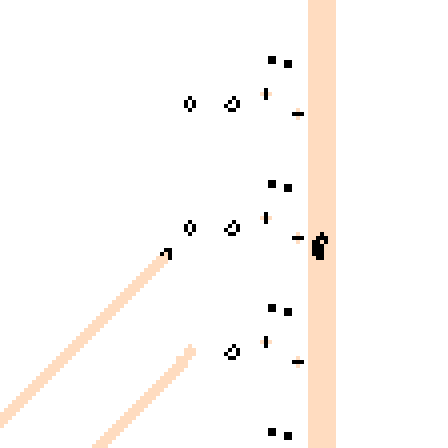
\includegraphics[width=2cm]{silverfish_synth9.png}};
			
			\filldraw[draw=gridgray,fill=white,line width=0.3pt,fill opacity=0.8] (\synninesmlx,\synninesmty) rectangle (\synninesmrx,\synninesmby);
			\draw[gridgray,line width=0.6pt] (\synninebglx,\synninebgty) rectangle (\synninebgrx,\synninebgby);
			
			\draw[gray] (\synninesmlx+0.1,\synninesmty-0.1) node {\tiny \texttt{9}};
			\draw[gray] (\synninebglx,\synninebgty) node[anchor=north west] {\small \texttt{9}};
		% END ZOOM SYNTH9
		
		% ZOOM BOX SYNTH10
			\newcommand\syntensmlx{4.33}
			\newcommand\syntensmrx{\syntensmlx+0.26}
			\newcommand\syntensmby{3.37}
			\newcommand\syntensmty{\syntensmby+0.2}
			
			\newcommand\syntenbglx{5.25}
			\newcommand\syntenbgrx{\syntenbglx+2}
			\newcommand\syntenbgty{5.375}
			\newcommand\syntenbgby{\syntenbgty-2}
			
			\node[inner sep=0pt,anchor=north west] (zooms10) at (\syntenbglx,\syntenbgty) {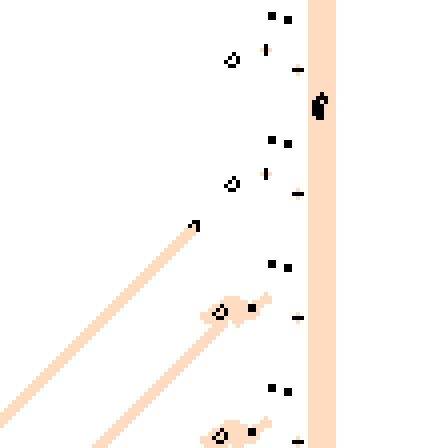
\includegraphics[width=2cm]{silverfish_synth10.png}};
			
			\filldraw[draw=gridgray,fill=white,line width=0.3pt,fill opacity=0.8] (\syntensmlx,\syntensmty) rectangle (\syntensmrx,\syntensmby);
			\draw[gridgray,line width=0.6pt] (\syntenbglx,\syntenbgty) rectangle (\syntenbgrx,\syntenbgby);
			
			\draw[gray] (\syntensmlx+0.13,\syntensmty-0.1) node {\tiny \texttt{10}};
			\draw[gray] (\syntenbglx,\syntenbgty) node[anchor=north west] {\small \texttt{10}};
		% END ZOOM SYNTH10
		
		% ZOOM BOX SYNTH11
			\newcommand\synelevensmlx{4.33}
			\newcommand\synelevensmrx{\synelevensmlx+0.26}
			\newcommand\synelevensmby{2.83}
			\newcommand\synelevensmty{\synelevensmby+0.2}
			
			\newcommand\synelevenbglx{7.625}
			\newcommand\synelevenbgrx{\synelevenbglx+2}
			\newcommand\synelevenbgty{5.375}
			\newcommand\synelevenbgby{\synelevenbgty-2}
			
			\node[inner sep=0pt,anchor=north west] (zooms11) at (\synelevenbglx,\synelevenbgty) {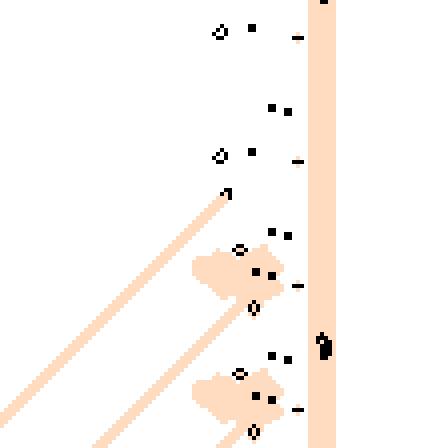
\includegraphics[width=2cm]{silverfish_synth11.png}};
			
			\filldraw[draw=gridgray,fill=white,line width=0.3pt,fill opacity=0.8] (\synelevensmlx,\synelevensmty) rectangle (\synelevensmrx,\synelevensmby);
			\draw[gridgray,line width=0.6pt] (\synelevenbglx,\synelevenbgty) rectangle (\synelevenbgrx,\synelevenbgby);
			
			\draw[gray] (\synelevensmlx+0.13,\synelevensmty-0.1) node {\tiny \texttt{11}};
			\draw[gray] (\synelevenbglx,\synelevenbgty) node[anchor=north west] {\small \texttt{11}};
		% END ZOOM SYNTH11
		
		% ZOOM BOX SYNTH12
			\newcommand\syntwelvesmlx{4.33}
			\newcommand\syntwelvesmrx{\syntwelvesmlx+0.26}
			\newcommand\syntwelvesmby{2.36}
			\newcommand\syntwelvesmty{\syntwelvesmby+0.2}
			
			\newcommand\syntwelvebglx{10}
			\newcommand\syntwelvebgrx{\syntwelvebglx+2}
			\newcommand\syntwelvebgty{5.375}
			\newcommand\syntwelvebgby{\syntwelvebgty-2}
			
			\node[inner sep=0pt,anchor=north west] (zooms12) at (\syntwelvebglx,\syntwelvebgty) {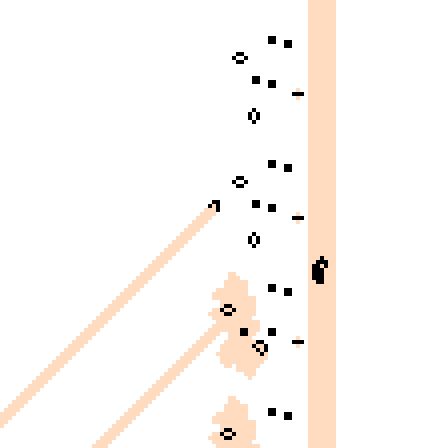
\includegraphics[width=2cm]{silverfish_synth12.png}};
			
			\filldraw[draw=gridgray,fill=white,line width=0.3pt,fill opacity=0.8] (\syntwelvesmlx,\syntwelvesmty) rectangle (\syntwelvesmrx,\syntwelvesmby);
			\draw[gridgray,line width=0.6pt] (\syntwelvebglx,\syntwelvebgty) rectangle (\syntwelvebgrx,\syntwelvebgby);
			
			\draw[gray] (\syntwelvesmlx+0.13,\syntwelvesmty-0.1) node {\tiny \texttt{12}};
			\draw[gray] (\syntwelvebglx,\syntwelvebgty) node[anchor=north west] {\small \texttt{12}};
		% END ZOOM SYNTH12
		
		% ZOOM BOX SYNTH13
			\newcommand\synthirsmlx{4.33}
			\newcommand\synthirsmrx{\synthirsmlx+0.26}
			\newcommand\synthirsmby{2.03}
			\newcommand\synthirsmty{\synthirsmby+0.2}
			
			\newcommand\synthirbglx{5.25}
			\newcommand\synthirbgrx{\synthirbglx+2}
			\newcommand\synthirbgty{3}
			\newcommand\synthirbgby{\synthirbgty-2}
			
			\node[inner sep=0pt,anchor=north west] (zooms13) at (\synthirbglx,\synthirbgty) {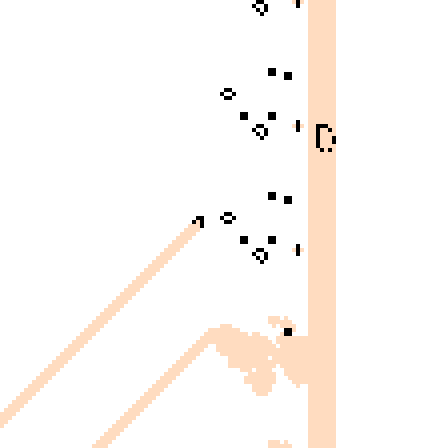
\includegraphics[width=2cm]{silverfish_synth13.png}};
			
			\filldraw[draw=gridgray,fill=white,line width=0.3pt,fill opacity=0.8] (\synthirsmlx,\synthirsmty) rectangle (\synthirsmrx,\synthirsmby);
			\draw[gridgray,line width=0.6pt] (\synthirbglx,\synthirbgty) rectangle (\synthirbgrx,\synthirbgby);
			
			\draw[gray] (\synthirsmlx+0.13,\synthirsmty-0.1) node {\tiny \texttt{13}};
			\draw[gray] (\synthirbglx,\synthirbgty) node[anchor=north west] {\small \texttt{13}};
		% END ZOOM SYNTH13
		
		% ZOOM BOX SYNTH14
			\newcommand\synfrteensmlx{4.33}
			\newcommand\synfrteensmrx{\synfrteensmlx+0.26}
			\newcommand\synfrteensmby{1.45}
			\newcommand\synfrteensmty{\synfrteensmby+0.2}
			
			\newcommand\synfrteenbglx{7.625}
			\newcommand\synfrteenbgrx{\synfrteenbglx+2}
			\newcommand\synfrteenbgty{3}
			\newcommand\synfrteenbgby{\synfrteenbgty-2}
			
			\node[inner sep=0pt,anchor=north west] (zooms14) at (\synfrteenbglx,\synfrteenbgty) {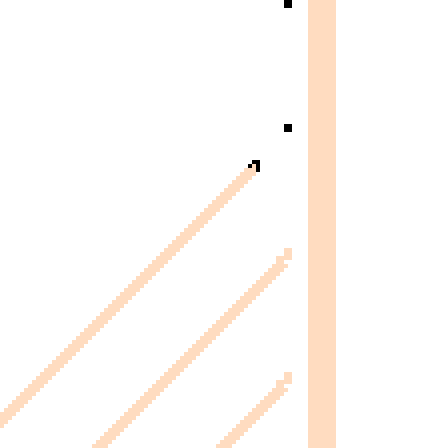
\includegraphics[width=2cm]{silverfish_synth14.png}};
			
			\filldraw[draw=gridgray,fill=white,line width=0.3pt,fill opacity=0.8] (\synfrteensmlx,\synfrteensmty) rectangle (\synfrteensmrx,\synfrteensmby);
			\draw[gridgray,line width=0.6pt] (\synfrteenbglx,\synfrteenbgty) rectangle (\synfrteenbgrx,\synfrteenbgby);
			
			\draw[gray] (\synfrteensmlx+0.13,\synfrteensmty-0.1) node {\tiny \texttt{14}};
			\draw[gray] (\synfrteenbglx,\synfrteenbgty) node[anchor=north west] {\small \texttt{14}};
		% END ZOOM SYNTH14
	\end{tikzpicture}
\end{document}